\documentclass[a4paper, 11pt, normalem]{report}

\usepackage{../../../LaTeX-Templates/Notes}
\usepackage{subfiles}
\usepackage{epigraph}
\usetikzlibrary{decorations.pathmorphing}
\usetikzlibrary{arrows.meta}

\tikzset{snake it/.style={decorate,decoration=snake}}
\tikzset{
    partial ellipse/.style args={#1:#2:#3}{
        insert path={+ (#1:#3) arc (#1:#2:#3)}
    }
}

\setlength{\epigraphwidth}{\textwidth}
\titleformat{\part}[display]
{\normalfont\huge\filcenter\bfseries\thispagestyle{epigraph}}
{\partname\ \thepart}
{20pt}
{\Huge}
\titlespacing*{\part}{0pt}{0pt}{40pt}

\title{Atoms, Lasers, and Qubits \vspace{-20pt}}
\author{Dr Weatheril and Prof Adams}
\date{\vspace{-15pt}Michaelmas Term 2019 - Epiphany Term 2020}
\rhead{\hyperlink{page.1}{Contents}}

\begin{document}

\maketitle
%\tableofcontents

\epigraphhead[200]{\hfil
\includegraphics[scale=0.5]{lasers.png}\hfil}
\part{}
\chapter{Introduction}
\begin{itemize}
    \item \textbf{Note:} The course will be more reading based than math based. 
Read the references on each summary sheet. 
    \item Need light oscillation, not just amplification.  
    \item 1 in $10^{18}$ atomic clock accuracy.
    \item LD: laser diode
    \item Non-linear crystals allow different wavelengths
    \item Laser transitions based on E group of materials
    \item Learn the unit conversions
    \item Magneto-optical trap to cool atoms
    \item Optical frequency comb $\to$ accurate measurement of wavelength of light 
    \item Sodium atoms in upper atmosphere which we fluoresce for AO
    \item \textbf{LEARN!} Q on paper always - contents of a laser
        \begin{enumerate}
            \item More in excited state than ground
            \item Pump gets energy in
            \item Mirrors to make light bounce back and forward
        \end{enumerate}
\end{itemize}

\section{Introduction to lasers}
Lasers - coherence $\to$ 2 types - longitudinal and transverse
\begin{itemize}
    \item Lasers are highly coherent, both transversely and longitudinally. 
        Longitudinal and temporal coherence is related to linewidth, and will be discussed. 
        Coherence length $l_c$ and coherence time $\tau_c$ are the distance and time over which a coherent wave maintains a specified degree of coherence, i.e. when its phase is predictable. 
\end{itemize}
\begin{multicols}{2}
\begin{figure}[H]
    \centering
    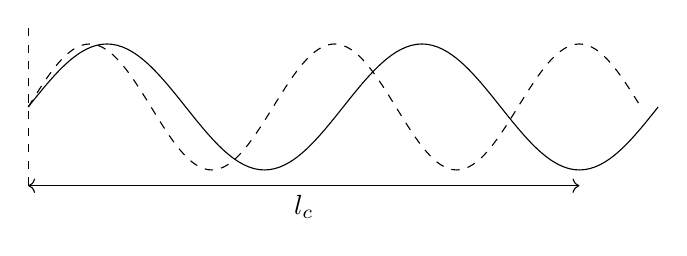
\begin{tikzpicture}
        \draw[dashed] (0,0) -- (0,2);
        \draw[<->] (0,0) -- (7,0) node[anchor=north,midway] {$l_c$};
        \draw (0,1) sin (1,1.8) cos (2,1) sin (3,0.2) cos (4,1) sin (5,1.8) cos (6,1) sin (7,0.2) cos (8,1);
        \draw[dashed] (0,1) sin (0.78,1.8) cos (1.56,1) sin (2.33,0.2) cos (3.11,1) sin (3.89,1.8) cos (4.67,1) sin (5.44,0.2) cos (6.22,1) sin (7,1.8) cos (7.78,1);
    \end{tikzpicture}
\end{figure}
\columnbreak
Coherence length and time:
\begin{align}
    l_c &= \frac{2\pi c}{\delta\om},~~  \tau_c = \frac{2\pi}{\delta\om}
\end{align}
\end{multicols}
\begin{itemize}
    \item Can't have an infinitely narrow spectrum. 
        Monochromaticity - laser has a spectral linewidth $\delta\om$, this is much smaller than the actual carrier/centre frequency. $\delta\om\ll\om_0$ for a laser where $\om_0$ is the centre frequency. 
        From mHz to GHz in range. 
    \item Highly directional beam $\to$ energy contained in one region. 
\end{itemize}
Directionality:
\begin{itemize}
    \item Lasers have highly directional beams that diverge due to diffraction
    \item Beam will be larger
    \item Waist of beam, $2\om_0$.
\end{itemize}
\begin{figure}[H]
    \centering
    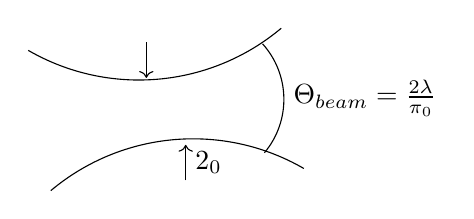
\begin{tikzpicture}
        \draw (0,1) arc (240:310:80pt);
        \draw (3.5,-0.5) arc (60:130:80pt);
        \draw (3,-0.3) arc (-40:42:30pt) node[anchor=west,midway] {$\Theta_{beam} = \frac{2\lambda}{\pi\om_0}$};
        \draw[->] (1.5,1.1) -- (1.5,0.65);
        \draw[->] (2,-0.65) -- (2,-0.2) node[anchor=west,midway] {$2\om_0$};
    \end{tikzpicture}
\end{figure}
\begin{itemize}
    \item All in a very low frequency range $\to$ all energy oscillating in small aarea in small frequency range - useful applications. 
\end{itemize}
Brightness:
\begin{itemize}
    \item Lasers are spectrally bright
    \item Definition of brightness - amount of power in particular area (solid angle) of the beam:
        \begin{equation}
            B_\om = \frac{P}{A\Delta\Om\Delta\om},
        \end{equation}
        where $A$ is the area, $\Delta\Om$ is the solid angle, and $\Delta\om$ is the linewidth. 
\end{itemize}
Electromagnetic Field Modes - not examinable:
\begin{itemize}
    \item 1st Chapter of 'Laser Physics' book
    \item Planck's radiation law
    \item Each unique solution of field is EM mode
    \item $L^3$ factored out when divided by volume
    \item Modes exist with or without energy
\end{itemize}


\chapter{Einstein's rate equations}
A laser requirs amplification due to stimulated emission of radiation. 
\begin{multicols}{2}
\begin{figure}[H]
    \centering
    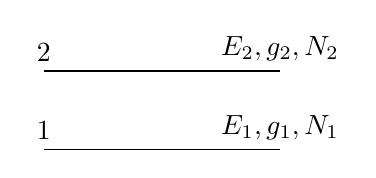
\begin{tikzpicture}
        \draw (0,1) node[anchor=south] {2} -- (3,1) node[anchor=south] {$E_2,g_2,N_2$};
        \draw (0,0) node[anchor=south] {1} -- (3,0) node[anchor=south] {$E_1,g_1,N_1$};
    \end{tikzpicture}
\end{figure}
\begin{align}
    E_2 - E_1 = \hbar\om_{12}
\end{align}
\end{multicols}
\begin{enumerate}
    \item Spontaneous emission: Atom in some excited state, until some time later where it spontaneously decays into a lower state, with a photon emitted with energy shown in Eq (2.1). 
        Rates: $A_{21}$ per $N_i$ atoms, or $A_{21}N_2$ per $m^3$.
        \begin{figure}[H]
            \centering
            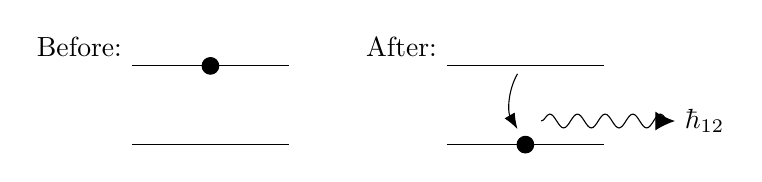
\begin{tikzpicture}
                \draw (0,1) node[anchor=south east] {Before:} -- (2,1);
                \draw[fill] (1,1) circle (3pt);
                \draw (0,0) -- (2,0);

                \draw (4,1) node[anchor=south east] {After:} -- (6,1);
                \draw (4,0) -- (6,0);
                \draw[fill] (5,0) circle (3pt);
                \draw[-{Latex[length=2mm,width=1.5mm]}] (4.9,0.9) arc (150:210:20pt);
                \draw[-{Latex[length=2.5mm,width=2.4mm]},snake it] (5.2,0.3) -- (6.9,0.3) node[anchor=west] {$\hbar\om_{12}$};
            \end{tikzpicture}
        \end{figure}
    \item Absorption: Excite into excited state using energy of photon. 
        Rates: $B_{12}\rho(\om_{12})$, $B_{12}\rho(\om_{12})N_2$.
        \begin{figure}[H]
            \centering
            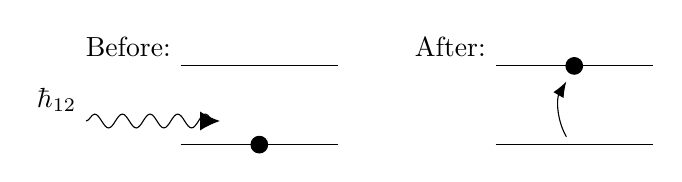
\begin{tikzpicture}
                \draw (0,1) node[anchor=south east] {Before:} -- (2,1);
                \draw[fill] (1,0) circle (3pt);
                \draw (0,0) -- (2,0);    
                \draw[-{Latex[length=2.5mm,width=2.4mm]},snake it] (-1.2,0.3) node[anchor=south east] {$\hbar\om_{12}$} -- (0.5,0.3);

                \draw (4,1) node[anchor=south east] {After:} -- (6,1);
                \draw (4,0) -- (6,0);
                \draw[fill] (5,1) circle (3pt);
                \draw[-{Latex[length=2mm,width=1.5mm]}] (4.9,0.1) arc (210:150:20pt);
            \end{tikzpicture}
        \end{figure}
    \item Stimulated emission: At the initial time we have an atom in an excited state which we then apply a radiated field (photon) to. Later, the atom will decay into a lower state and there will be two outgoing photons - they have been emitted into the same mode.
        Rates: $B_{21}\rho(\om_{12})$, $B_{21}\rho(\om_{12})N_2$. Note: 
        \begin{itemize}
            \item Here, $\rho(\om_{12})$ is the spectral energy density - the energy density, per unit angular frequency range at $\om$, with units of $J\,m^{-3}\,s$.
            \item Generally, the light being used here is broad-band.
        \end{itemize}
        \begin{figure}[H]
            \centering
            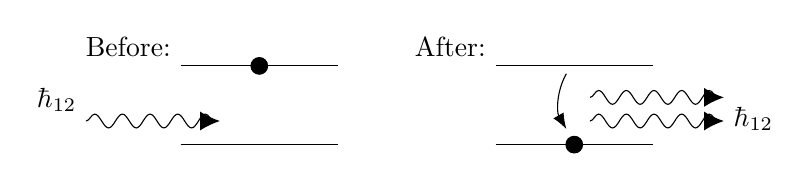
\begin{tikzpicture}
                \draw (0,1) node[anchor=south east] {Before:} -- (2,1);
                \draw[fill] (1,1) circle (3pt);
                \draw (0,0) -- (2,0);    
                \draw[-{Latex[length=2.5mm,width=2.4mm]},snake it] (-1.2,0.3) node[anchor=south east] {$\hbar\om_{12}$} -- (0.5,0.3);
                
                \draw (4,1) node[anchor=south east] {After:} -- (6,1);
                \draw (4,0) -- (6,0);
                \draw[fill] (5,0) circle (3pt);
                \draw[-{Latex[length=2mm,width=1.5mm]}] (4.9,0.9) arc (150:210:20pt);
                \draw[-{Latex[length=2.5mm,width=2.4mm]},snake it] (5.2,0.3) -- (6.9,0.3);
                \draw[-{Latex[length=2.5mm,width=2.4mm]},snake it] (5.2,0.6) -- (6.9,0.6) node[anchor=north west] {$\hbar\om_{12}$};
            \end{tikzpicture}
        \end{figure}
\end{enumerate}

\section{Apply the 3 processess}
\begin{figure}[H]
    \centering
    \begin{tikzpicture}
        \draw (0.5,2) node[anchor=south east] {2} -- (7.5,2) node[anchor=south west] {$E_2$};
        \draw (0.5,0) node[anchor=north east] {1} -- (7.5,0) node[anchor=north west] {$E_1$};
        \draw[-{Latex[length=2mm,width=1.5mm]}] (2,2) -- (2,0) node[anchor=east,midway] {$A_{21}$};
        \draw[-{Latex[length=2mm,width=1.5mm]}] (4,0) -- (4,2) node[anchor=east,midway] {$B_{12}\rho(\om_{12})$};
        \draw[-{Latex[length=2mm,width=1.5mm]}] (6,2) -- (6,0) node[anchor=east,midway] {$B_{21}\rho(\om_{12})$};
    \end{tikzpicture}
\end{figure}
Conservation of atom number:
\begin{align}
    \frac{dN_2}{dt} &= -\frac{dN_1}{dt} \\
    N_1 + N_2 &= N = \text{const} \\
    N_1B_{12}\rho(\om_{12}) &= N_2A_{21} + N_2B_{21}\rho(\om_{12})
\end{align}
Rearrange for the spectral energy density:
\begin{align}
    \rho(\om_{12}) &= \frac{N_2A_{21}}{N_1B_{12}-N_2B_{21}} = \frac{\frac{A_{21}}{B_{21}}}{\frac{N_1}{N_2}\frac{B_{12}}{B_{21}} - 1}
\end{align}
Substitute using Boltzmann Law:
\begin{align}
    \frac{N_2}{N_1} &= \frac{g_2}{g_1}\exp\left(-\frac{\hbar\om_{12}}{k_BT}\right) \\
    \implies \rho(\om_{12}) &= \frac{\frac{A_{21}}{B_{21}}}{\frac{g_1}{g_2}\frac{B_{12}}{B_{21}}\exp\left(\frac{\hbar\om_{12}}{k_BT}\right) - 1}
\end{align}
Now look at Planck's Law:
\begin{align}
    \rho(\om) &= \frac{\hbar\om^3}{\pi^2c^3} \frac{1}{\exp\left(\frac{\hbar\om}{k_BT}\right) - 1}
\end{align}
Einstein realised there must be an extra condition to switch between these two forms.
This reveals:
\begin{align}
    g_1B_{12} &= g_2B_{21} \\
    A_{21} &= \frac{\hbar\om_{12}^3}{\pi^2c^3}B_{21}
\end{align}
Notes:
\begin{itemize}
    \item Effectively only 1 coefficient as if we know A, we know B. 
    \item $A_{21}$ is the radiative decay rate,
        \begin{equation}
            A_{21} = \frac{1}{\tau_2}
        \end{equation}
    \item B has units $m^3\,J^{-1}\,s^{-2}$.
    \item A and B are constants for a particular atom.
    \item From the $\om^3$ term, we can see that an infrared transition may decay very fast, but a microwave transition may decay very slow. 
    \item Ratio of $A/B \propto \om^3$ - lasers at high requency harder to achieve.
    \item The principle of detailed balance states that \textbf{\unl{in equilibrium}, the total number of particles entering a quantum state by a partucular rate per unit time is the same as the number leaving by the same rate.}
\end{itemize}

\section{Steady State Solution}
For simplicity, we will assume that $g_1=g_2$ such that the B coefficients are the same. 
\begin{align}
    N_1B_{12}\rho(\om_{12}) &= N_2A_{21} + N_2B_{12}\rho(\om_{12}) \\
    N_1 &= N - N_2
\end{align}
Now we can rearrange to eliminate $N_1$.
\begin{align}
    \frac{N_2}{N} &= \frac{B_{12}\rho(\om_{12})}{A_{21}+2B_{12}\rho(\om_{12})}
\end{align}
Now consider the form of the above as the spectral energy density tends to infinity. 
What we see  is that $N_2 \to \frac{N}{2}$.
This tells us that for at least a two-level atom we cannot get population inversion, which is required for lasers, i.e. steady state inversion impossible.

\section{Number of photons per mode}
$\bar{n}$ can be thought of as the mean number of photons per mode, and $g(\om)\,d\om$ as the mode density. 
\begin{align}
    \rho(\om)\,d\om &= \bar{n} \times g(\om)\,d\om \times \hbar\om
\end{align}
Standard result:
\begin{align}
    g(\om)\,d\om &= \frac{\om^2}{\pi^2c^3}\,d\om \\
    \implies \bar{n} &= \frac{\rho(\om)}{\hbar\om g(\om)} = \frac{\pi^2c^3}{\hbar\om^3}\rho(\om)\\
    \bar{n} &= \frac{B_{21}\rho(\om)}{A_{21}} = \frac{\text{rate of stimulated emission}}{\text{rate of spontaneous emission}}
\end{align}
It follows that:
\begin{itemize}
    \item $\bar{n}>1$ - stimulated emission dominates $\implies$ LASERS
    \item $\bar{n}<1$ - spontaneous emission dominates $\implies$ classical light source
\end{itemize}
For a black body:
\begin{align}
    \bar{n} &= \frac{1}{\exp\left(\frac{\hbar\om_{12}}{k_BT}\right) -1} = \frac{B_{12}\rho(\om)}{A_{21}}
\end{align}
These rates are equal when
\begin{align}
    \frac{\hbar\om_{12}}{k_BT} &= \ln(2)
\end{align}
For $\lambda=500\,nm$, $T= 41400\,K$. So for most black bodies, stimulated emission is negligible.

\chapter{Linewidths and Lineshapes}
2 types of broadening:
\begin{itemize}
    \item Homogeneous - all atoms in sample affected the same
    \item Inhomogeneous - atoms in sample affected differently
\end{itemize}

\section{Homogeneous Broadening}
Every atom/molecule exhibits this type of broadening to varying magnitudes.\\
\textbf{Radiative (natural) broadening:}
\begin{itemize}
    \item Consider some excited state population, $N_2$. $e^{-\Gamma_Ht}$
        Leads to some spread in maximum.
        \begin{equation}
            FWHM = \Gamma_H
        \end{equation}
        This broadening follows from the Heisenberg uncertainty principle: Finite lifetime $\implies$ spread in energy, $\Delta E\Delta t \approx \hbar/2$, then a spread in energy $\implies$ a spread in frequency,
        \begin{equation}
            \Delta E = \hbar\Delta\om \implies \Delta\om = \frac{1}{\tau_2} = A_{21} = \Gamma_H
        \end{equation}
        This is only for a 2 level atom.
        \begin{figure}[H]
            \centering 
            \begin{tikzpicture}
                \draw[->] (0,0) -- (0,2) node[anchor=east] {$N_2$};
                \draw[->] (0,0) -- (3,0) node[anchor=west] {$t$};
                \draw (0.2,2) .. controls (0.5,1) and (1.5,0.3) .. (3,0.2) node[anchor=south west] {$e^{-\Gamma_Ht}$};

                \draw[->] (5,0) -- (9,0) node[anchor=west] {$\om$}; 
                \draw (7,-0.1) node[anchor=north] {$\om_{12}$} -- (7,0.1);
                \draw (5.1,0.1) cos (6.7,1.7) sin (7,2) cos (7.3,1.7) sin (8.9,0.1);
                \draw[<->] (6.3,1) -- (7.7,1) node[anchor=south west] {FWHH $= \Gamma_H$};
            \end{tikzpicture}
        \end{figure}
    \item Define the normalised lineshape function:
        \begin{align}
            L_H(\om) &= \frac{\Gamma_H/2\pi}{(\om-\om_{12})^2+\frac{\Gamma_H^2}{4}} \\
            \ofnt &L_H(\om)\;d\om = 1
        \end{align}
    \item For multiple decay paths: 
        \begin{multicols}{2}
        \begin{figure}[H]
            \centering
            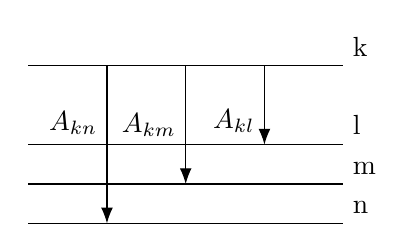
\begin{tikzpicture}
                \draw (0,2) -- (4,2) node[anchor=south west] {k};
                \draw (0,1) -- (4,1) node[anchor=south west] {l};
                \draw (0,0.5) -- (4,0.5) node[anchor=south west] {m};
                \draw (0,0) -- (4,0) node[anchor=south west] {n};

                \draw[-{Latex[length=2mm,width=1.5mm]}] (1,2) -- (1,0) node[anchor= south east,midway] {$A_{kn}$};
                \draw[-{Latex[length=2mm,width=1.5mm]}] (2,2) -- (2,0.5) node[anchor=east,midway] {$A_{km}$};
                \draw[-{Latex[length=2mm,width=1.5mm]}] (3,2) -- (3,1) node[anchor=north east,midway,yshift=2pt] {$A_{kl}$};
            \end{tikzpicture}
        \end{figure}
        For level k
        \begin{align}
            \frac{dN_k}{dt} &= -N_kA_{kl} - N_kA_{km} - N_kA_{kn} \\
            \tau_k &= \frac{1}{\sum A_{ki}} = \frac{1}{\Gamma_H}
        \end{align}
        \end{multicols}
    \item When both levels decay:
        \begin{figure}[H]
            \centering
            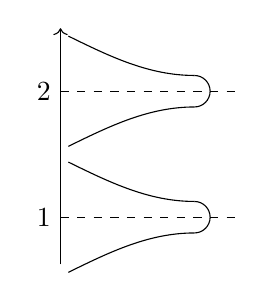
\begin{tikzpicture}
                \draw[->] (0,0) -- (0,3);
                \draw (0.1,2.9) sin (1.7,2.4);
                \draw (1.7,2.4) arc (90:-90:0.2cm);
                \draw (1.7,2) cos (0.1,1.5);
                
                \draw (0.1,1.3) sin (1.7,0.8);
                \draw (1.7,0.8) arc (90:-90:0.2cm);
                \draw (1.7,0.4) cos (0.1,-0.1);

                \draw[dashed] (0,2.2) node[anchor=east] {2} -- (2.3,2.2);
                \draw[dashed] (0,0.6) node[anchor=east] {1} -- (2.3,0.6);
            \end{tikzpicture}
        \end{figure}
        \begin{align}
            \Gamma_2 &= \sum A_{2i} = \frac{1}{\tau_2} \\
            \Gamma_1 &= \sum A_{1i} = \frac{1}{\tau_1} \\
            \Gamma_{21} &= \Gamma_2 + \Gamma_1
        \end{align}
        $\Gamma_{21}$ is the emission linewidth. 
\end{itemize}
\begin{example}[Argon ion laser]
    \begin{figure}[H]
        \centering
        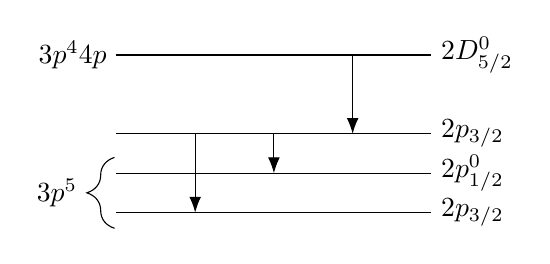
\begin{tikzpicture}
            \draw (0,2) node[anchor=east] {$3p^44p$} -- (4,2) node[anchor=west] {$2D_{5/2}^0$};
            \draw (0,1) -- (4,1) node[anchor=west] {$2p_{3/2}$};
            \draw (0,0.5) -- (4,0.5) node[anchor=west] {$2p_{1/2}^0$};
            \draw (0,0) -- (4,0) node[anchor=west] {$2p_{3/2}$};

            \draw[-{Latex[length=2mm,width=1.5mm]}] (3,2) -- (3,1);
            \draw[-{Latex[length=2mm,width=1.5mm]}] (2,1) -- (2,0.5);
            \draw[-{Latex[length=2mm,width=1.5mm]}] (1,1) -- (1,0);

            \draw[decorate,decoration={brace,amplitude=10pt},xshift=5pt] (-0.2,-0.2) -- (-0.2,0.7) node[midway,anchor=east,xshift=-10pt] {$3p^5$}; 
        \end{tikzpicture}
    \end{figure}
    $\lambda = 488\,nm$, $A= 7.8\times10^7\;s^{-1}$, $1:\,73,1\;nm;~ A=4.5\times10^8\;s^{-1}$, $2:\,72.3\;nm;~ A=23\times10^8\;s^{-1}$.\\
    Emission linewidth:
    \begin{align}
        \sum A &= 2.8\times10^9 = (2\pi)450\;MHz
    \end{align}
\end{example}
\textbf{Collisional/pressure broadening:}
\begin{itemize}
    \item Collisions between atoms - de-excite the atoms $\to$ reduce excited state lifetime $\to$ broader transition
    \item Depends on pressure - important for gas lasers
\end{itemize}
\textbf{Phonon broadening:}
\begin{itemize}
    \item \textit{doodle of standard 1,2 transition for bare atom/ion}. In a crystal, two distinct groups of energy levels packed together, quantised vibrational modes $\implies$ phonons. 
    \item Occurs in solid state lasers, and is temperature tempendent
    \item Dominant broadening at room temperature
\end{itemize}

\section{Inhomogeneous Broadening}
\textbf{Doppler Broadening:}
\begin{itemize}
    \item Arises due to motion of atoms - when a moving atom emits, there is a Doppler shift dependent on the component of velocity along the direction of the emitted photon.
        \begin{align}
            \om &= \om_{12}\left(1 \pm \frac{v_z}{c}\right)
        \end{align} 
        $\pm$ for blue/red shift - blue as velocity towards observer, red away. 
    \item Broadening arises due to Maxwell-Boltzmann distribution of velocities,
        \begin{align}
            P(v_z)\,dv_z &= \left(\frac{M}{2\pi k_BT}\right)^{1/2} \exp\left(-\frac{Mv_z^2}{2k_BT}\right)\;dv_z
        \end{align}
        Use correspondence between $v_z$ and $\om$ to get
        \begin{figure}[H]
            \centering
            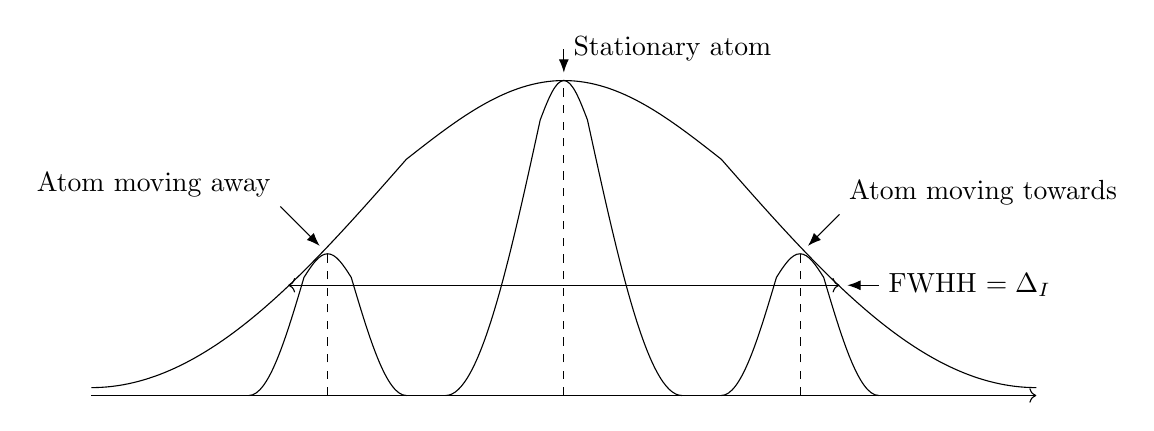
\begin{tikzpicture}
                \draw[->] (0,0) -- (12,0);
                \draw (0,0.1) cos (4,3) sin (6,4) cos (8,3) sin (12,0.1);
                \draw (2,0) cos (2.7,1.5) sin (3,1.8) cos (3.3,1.5) sin (4,0);
                \draw (4.5,0) cos (5.7,3.5) sin (6,4) cos (6.3,3.5) sin (7.5,0);
                \draw (8,0) cos (8.7,1.5) sin (9,1.8) cos (9.3,1.5) sin (10,0);

                \draw[dashed] (3,0) -- (3,1.8);
                \draw[dashed] (6,0) -- (6,4);
                \draw[dashed] (9,0) -- (9,1.8);

                \draw[<->] (2.5,1.4) -- (9.5,1.4);
                \draw[-Latex] (10,1.4) node[anchor=west] {FWHH $= \Delta\om_I$} -- (9.6,1.4);
                \draw[-Latex] (9.5,2.3) node[anchor=south west] {Atom moving towards} -- (9.1,1.9);
                \draw[-Latex] (2.4,2.4) node[anchor=south east] {Atom moving away} -- (2.9,1.9);
                \draw[-Latex] (6,4.4) node[anchor=west] {Stationary atom} -- (6,4.1);
            \end{tikzpicture}
        \end{figure}
        \begin{align}
            P(\om)\,d\om &= \frac{c}{\om_{12}}\left(\frac{M}{2\pi k_BT}\right)^{1/2}\exp\left[-\frac{Mc^2}{2k_B T}\frac{(\om-\om_{12})^2}{\om_{12}^2}\right]
        \end{align}
    \item For Doppler broadening, 
        \begin{align}
            \Delta\om_I &= \frac{2\om_{12}}{c}\left(\frac{2k_BT}{M}\ln2\right)^{1/2} \\
                        &= 7.16\times10^{-7}\om_{12}\left(\frac{T}{M_A}\right)^{1/2}
        \end{align}
        $\Delta\om_I$ is known as the Doppler width, $M_A$ is using the mass in atomic units instead of kg as used so far for $M$.
\end{itemize}
\begin{example}[Argon ion laser 2]
$M_A = 40$, $\lambda=488\,nm$, Discharge temperature $\approx 1200^\circ C$.
\begin{align}
    \Delta\om_I &= (2\pi) 2.7\,GHz
\end{align}
This is many times larger than the natural broadening. 
\end{example}
\textbf{Amorphous crystal broadening:}
\begin{itemize}
    \item Occurs in glass materials
    \item Inhomogeneities are Gaussian (normal), the emission is also Gaussian
\end{itemize}

\chapter{Amplification by Stimulated Emission}
\begin{example}
\begin{figure}[H]
    \centering
    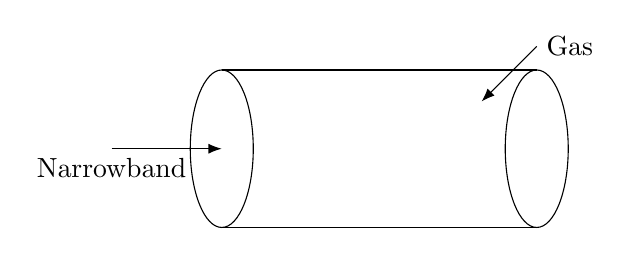
\begin{tikzpicture}
        \draw (0,0) ellipse (0.4cm and 1cm);
        \draw (0,1) -- (4,1);
        \draw (0,-1) -- (4,-1);
        \draw (4,0) ellipse (0.4cm and 1cm);
        \draw[-Latex] (4,1.3) node[anchor=west] {Gas} -- (3.3,0.6);

        \draw[-Latex] (-1.4,0) node[anchor=north] {Narrowband} -- (0,0);
    \end{tikzpicture}
\end{figure}
If the light beam is resonant with the atoms in the gas, we would expect some interaction. 
But how is the medium excited?
It depends on the broadening. 
\begin{enumerate}
    \item Homogeneous broadening (Lorentzian):
        \begin{figure}[H]
            \centering
            \begin{tikzpicture}
                \draw[->] (-3,0) -- (3,0) node[anchor=north] {$\om$};
                \draw[->] (0,0) node[anchor=north] {$\om_{12}$} -- (0,4) node[anchor=east] {$N_1$};
                \draw (-2.8,0.1) cos (-0.4,3.2) sin (0,3.8) cos (0.4,3.2) sin (2.8,0.1);

                \draw[-Latex] (3,2) -- (4,2);

                \draw[->] (4,2.5) -- (10,2.5) node[anchor=north] {$\om$};
                \draw[->] (7,2.5) node[anchor=north] {$\om_{12}$} -- (7,4.5) node[anchor=east] {$N_2$};
                \draw[dashed] (4.2,2.6) cos (6,3.5) sin (7,3.8) cos (8,3.5) sin (9.8,2.6);

                \draw[->] (4,-1) -- (10,-1) node[anchor=north] {$\om$};
                \draw[->] (7,-1) node[anchor=north] {$\om_{12}$} -- (7,2) node[anchor=east] {$N_1$};
                \draw (4.2,-0.8) cos (6.4,1.2) sin (7,1.8) cos (7.6,1.2) sin (9.8,-0.8);
                \draw[dashed] (4.2,-0.9) cos (6.4,0.8) sin (7,1.4) cos (7.6,0.8) sin (9.8,-0.9);
            \end{tikzpicture}
        \end{figure}
        Turn on radiation within natural linewidth. 
        All of these distributions will be the same - all atoms are affected equally, and the population of $N_1$ is reduced slightly as it moves into $N_2$.
    \item Inhomogeneous broadening (Gaussian): 
        \begin{figure}[H]
            \centering
            \begin{tikzpicture}
                \draw[->] (-3,0) -- (3,0) node[anchor=north] {$\om$};
                \draw[->] (0,0) node[anchor=north] {$\om_{12}$} -- (0,3) node[anchor=east] {$N_1$};
                \draw (-2.8,0.1) cos (-1,2) sin (0,2.8) cos (1,2) sin (2.8,0.1);
                \draw[fill] (0.75,0) rectangle (1.25,0.6);

                \draw[-Latex] (3,1.5) -- (4,1.5);

                \draw[->] (4,2.5) -- (10,2.5) node[anchor=north] {$\om$};
                \draw[->] (7,2.5) node[anchor=north] {$\om_{12}$} -- (7,3.5) node[anchor=east] {$N_2$};
                \draw[dashed] (7.5,2.5) cos (7.9,3) sin (8,3.2) cos (8.1,3) sin (8.5,2.5);

                \draw[->] (4,-1) -- (10,-1) node[anchor=north] {$\om$};
                \draw[->] (7,-1) node[anchor=north] {$\om_{12}$} -- (7,2) node[anchor=east] {$N_1$};
                \draw (4.1,-0.9) cos (6,0.8) sin (7,1.5) cos (7.5,1) sin (8,-0.2) cos (8.5,0.2) sin (9.9,-0.9);
            \end{tikzpicture}
        \end{figure}
        Distributions are now very different - atoms are affected differently, and only a subset of the atoms interact.
        For example, with Doppler broadening, only particles with a specific velocity would be excited strongly by the light beam. 
        The width of the N2 Gaussian is determined by natural broadening. 
\end{enumerate}
\end{example}
Reminder:
\begin{align}
    A_{21}N_2 &\equiv \text{rate of spontaneous emission per }m^3 \\
    B_{12}\rho(\om_{12})N_1 &\equiv \text{rate of absorption per }m^3 \\
    B_{21}\rho(\om_{12})N_2 &\equiv \text{rate of stimulated emission per }m^3
\end{align}
\section{Homogeneous broadening}
All atoms are affected the same $\implies$ simply define a new constant:
\begin{align}
    a_{21}(\om) &= A_{21}L_H(\om) & b_{12}(\om) &= B_{12}L_H(\om) & b_{21}(\om) &= B_{21}L_H(\om)
\end{align}
Then if we wanted to know the rate of emission now:
\begin{align}
    a_{21}(\om)\,d\om &= \text{rate of emission in range $\om\to\om+d\om$ per atom} 
\end{align}
We have to multiply by the $d\om$ because $L_H(\om)$ has units $\frac{1}{\om}$.
Integrating recovers the result,
\begin{align}
    \int L_H(\om)\,d\om &= 1
\end{align}
Inhomogeneous broadening is more difficult. 
We want to do this, but we can use the results from homogeneous broadening in certain circumstances, i.e. for narrowband light and $\Gamma_H \ll \Delta\om_I$.

\begin{figure}[H]
    \centering
    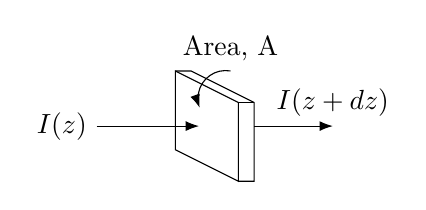
\begin{tikzpicture}
        \draw (0,0) -- (0.8,-0.4) -- (0.8,0.6) -- (0,1) -- cycle;
        \draw (0.8,-0.4) -- (1,-0.4) -- (1,0.6) -- (0.2,1) -- (0,1);
        \draw (1,0.6) -- (0.8,0.6);

        \draw[-Latex] (-1,0.3) node[anchor=east] {$I(z)$} -- (0.3,0.3);
        \draw[-Latex] (1,0.3) -- (2,0.3) node[anchor=south] {$I(z+dz)$};
        \draw[-Latex] (0.7,1) node[anchor=south] {Area, A} arc (80:200:10pt);
    \end{tikzpicture}
\end{figure}
Consider a \unl{weak} narrowband beam of light, frequency $\om$ and bandwidth $d\om$. \\
Assume:
\begin{itemize}
    \item No spontaneous emission
    \item Homogeneous broadening
    \item Steady state
\end{itemize}
Find change in power of beam.
\begin{align}
    \left(I(z+dz) - I(z)\right)A &= \left[N_2B_{21}L_H(\om)\rho(\om_{12})\,d\om - N_1B_{12}L_H(\om)\rho(\om_{12})\,d\om\right]\times\hbar\om\times A\,dz
\end{align}
The term inside the square brackets above is the net rate of photons added to the field ($m^{-3}$).\\
For a beam, the intensity is described as
\begin{align}
    I(z) &= c\rho(\om)\;d\om 
\end{align}
Substitute this into Eq (4.7) and rearrange, also using the expressions for A and B coefficients found in lecture 2: 
\begin{align}
    \frac{1}{I}\frac{dI}{dz} &= \frac{\hbar\om}{c}L_H(\om)\left[N_2B_{21} - N_1B_{12}\right] \\
                             &= \frac{\pi^2c^2}{\om^2_{12}}A_{21}L_H(\om)\left[N_2 - \frac{g_2}{g_1}N_1\right]
\end{align}
This uses the assumption that we are close to resonance.\\
The prefactor can be defined as the optical gain cross section,
\begin{align}
    \sigma(\om) &= \frac{\pi^2c^2}{\om_{12}^2}A_{21}L_H(\om).
\end{align}
Solve equation:
\begin{align}
    I(z) &= I(0)\exp\left[\sigma(\om)\times\left(N_2-\frac{g_2}{g_1}N_1\right)z\right]
\end{align}
There are two cases:
\begin{enumerate}
    \item Absorption:
        \begin{align}
            N_2 &< \frac{g_2}{g_1}N_1 \\
            \implies I(z) &= I(0)e^{-\kappa(\om)z},~ \kappa(\om) = \sigma(\om)\left(\frac{g_2}{g_1}N_1 - N_2\right)  
        \end{align}
        $\kappa$ is the absorption coefficient. 
        \begin{figure}[H]
            \centering
            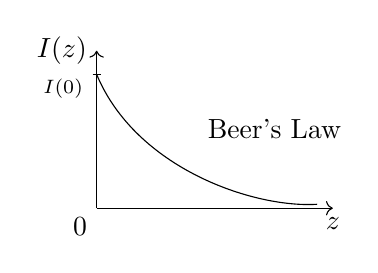
\begin{tikzpicture}
                \draw[->] (0,0) -- (0,2) node[anchor=east] {$I(z)$};
                \draw[->] (0,0) node[anchor=north east] {0} -- (3,0) node[anchor=north] {$z$};
                \draw (0,1.7) .. controls (0.5,0.5) and (2,0) .. (2.8,0.05) node[anchor=south west,midway,yshift=10pt] {Beer's Law};
                \draw (-0.05,1.7) node[anchor=east,yshift=-5pt] {\scriptsize $I(0)$} -- (0.05,1.7);
            \end{tikzpicture}
        \end{figure}
    \item Amplification.
        \begin{align}
            N_2 &> \frac{g_2}{g_1}N_1 \\
            I(z) &= I(0)e^{g(\om)z},~ g(\om) = \sigma(\om)\left(N_2-\frac{g_2}{g_1}N_1\right)
        \end{align}
        $g(\om)$ is the gain coefficient, $e^{g(\om)z}$ is the gain. 
        \begin{figure}[H]
            \centering
            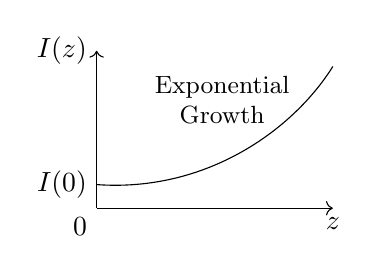
\begin{tikzpicture}
                \draw[->] (0,0) -- (0,2) node[anchor=east] {$I(z)$};
                \draw[->] (0,0) node[anchor=north east] {0} -- (3,0) node[anchor=north] {$z$};
                \draw (0,0.3) node[anchor=east] {$I(0)$} .. controls (1.4,0.2) and (2.5,1) .. (3,1.8) node[anchor=north,xshift=-40pt] {\small \shortstack{Exponential \\ Growth}};
            \end{tikzpicture}
        \end{figure}
\end{enumerate}
The condition for gain is
\begin{equation}
    N_2 > \frac{g_2}{g_1}N_1.
\end{equation}
This is known as \unl{Population Inversion.}
Frequency dependence of the gain:
\begin{align}
    g(\om) &= \sigma(\om)\times N^*, ~ N^* = N_2 - \frac{g_2}{g_1}N_1 \\
           &= \frac{\pi^2c^2}{\om_{12}^2}A_{21}L_H(\om)\times \left[N_2-\frac{g_2}{g_1}N_1\right]
\end{align}
We call $N^*$ the population inversion density. 
\textbf{Note:} Frequency dependence is in the optical gain cross section via $L(\om)$. 
$\sigma(\om)$ is determined by the atom, we cannot control it. 
Broadening spreads gain over a range of frequencies. 

\chapter{The Laser Oscillator: Cavity Basics and Threshold}
\begin{figure}[H]
    \centering
    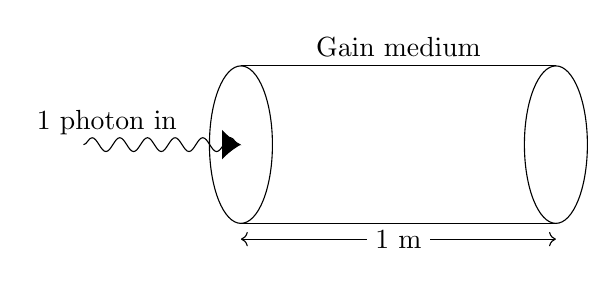
\begin{tikzpicture}
        \draw[-{Latex[length=2.4mm,width=3.8mm]},snake it] (-1,0) -- (1,0) node[anchor=south,midway,xshift=-20pt] {1 photon in};
        \draw (5,0) ellipse (0.4cm and 1cm);
        \draw (1,0) ellipse (0.4cm and 1cm);
        \draw (1,1) -- (5,1) node[anchor=south,midway] {Gain medium};
        \draw (1,-1) -- (5,-1);
        \draw[->] (2.6,-1.2) -- (1,-1.2);
        \draw[->] (3.4,-1.2) -- (5,-1.2);
        \draw[white] (2.6,-1.2) -- (3.4,-1.2) node[midway,black] {1 m};
    \end{tikzpicture}
\end{figure}
Imagine we have a sample which is our laser gain sample, and we will send one photon in. 
For most lasers,  the peak gain, $g(\om_{12}) \approx 0.01\;cm^{-1}$.
So one photon in to our 1m long sample, means $e^1 = 2.7$ photons out.
We must add a cavity to recirculate the light, and now using mirrors either side of the gain medium,  we will pass through the gain medium 40 times, $e^{40} \approx 10^{17}$ photons.
\begin{figure}[H]
    \centering
    \begin{tikzpicture}
        \draw (0,3) arc (120:240:40pt);
        \draw (4,3) arc (60:-60:40pt);
        \draw[-Latex] (0.5,1.6) arc (315:60:0.3cm);
        \draw (1,1.25) rectangle (3,2.25);
        \draw[-Latex] (3.5,2.05) arc (135:-120:0.3cm);
    \end{tikzpicture}
\end{figure}

\section{General Cavity Design}
\begin{figure}[H]
    \centering
    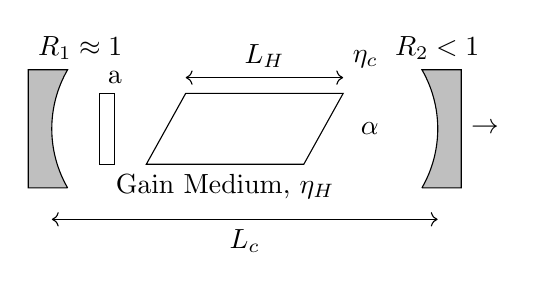
\begin{tikzpicture}
        \filldraw[fill=lightgray,draw=black] (0,0) -- (-0.5,0) -- (-0.5,1.5) node[anchor=south west] {$R_1 \approx 1$} -- (0,1.5) arc (150:210:1.5cm);
        \filldraw[fill=lightgray,draw=black] (4.5,0) -- (5,0) -- (5,1.5) node[anchor=west,midway] {$\to$} node[anchor=south east,xshift=10pt] {$R_2 < 1$} -- (4.5,1.5) arc (30:-30:1.5cm);

        \draw (1,0.3) -- (3,0.3) node[anchor=north,midway] {Gain Medium, $\eta_H$} -- (3.5,1.2) node[anchor=west,midway,xshift=10pt] {$\alpha$} -- (1.5,1.2) -- cycle;
        \draw (0.4,0.3) rectangle (0.6,1.2) node[anchor=south] {a};

        \draw[<->] (1.5,1.4) -- (3.5,1.4) node[anchor=south,midway] {$L_H$} node[anchor=south west] {$\eta_c$};
        \draw[<->] (-0.2,-0.4) -- (4.7,-0.4) node[anchor=north,midway] {$L_c$};
    \end{tikzpicture}
\end{figure}
\begin{itemize}
    \item $R_1$ is mirror 1 and must have a reflectivity as close to 1 as possible
    \item $R_2$ is the output coupler and must have a lower reflectivity so that the laser can eventually escape through this
    \item $L_c$ is the mirror separation, the length of the cavity
    \item $\alpha$ is the distributed loss over the length of the gain medium
    \item a is the intracavity element - it can make pulsed lasers or change the frequency, or induce a fixed loss
    \item The gain cell is angled, cut at Brewster's angle to minimise loss. 
    \item The cavity imposes spectrum and characteristics to the laser. 
    \item Distributed loss throughout cavity of $\alpha$ per meter.
\end{itemize}

\section{Longitudinal Cavity Modes}
The field in the cavity forms standing waves, i.e.
\begin{equation}
    n\frac{\lambda_n}{2} = L_c
\end{equation}
$n$ is called the mode order.
Mode separation,
\begin{equation}
    \Delta\nu_{fsr} = \nu_{n+1} - \nu_n = \frac{c}{2L_c}
\end{equation}
This is the \unl{Free Spectral Range.}
\begin{example}[Mode order of 10cm cavity at $\lambda= 500\,nm$]
\begin{wrapfigure}{l}{0.5\textwidth}
    \centering
    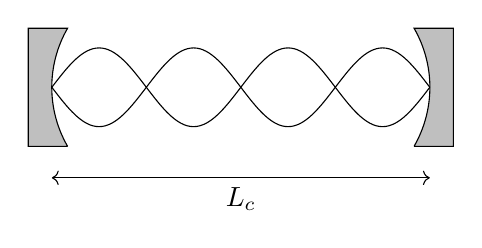
\begin{tikzpicture}
    \filldraw[fill=lightgray,draw=black] (0,0) -- (-0.5,0) -- (-0.5,1.5) -- (0,1.5) arc (150:210:1.5cm);
    \filldraw[fill=lightgray,draw=black] (4.4,0) -- (4.9,0) -- (4.9,1.5) -- (4.4,1.5) arc (30:-30:1.5cm);
    \draw (-0.2,0.75) sin (0.4,1.25) cos (1,0.75) sin (1.6,0.25) cos (2.2,0.75) sin (2.8,1.25) cos (3.4,0.75) sin (4,0.25) cos (4.6,0.75);
    \draw (-0.2,0.75) sin (0.4,0.25) cos (1,0.75) sin (1.6,1.25) cos (2.2,0.75) sin (2.8,0.25) cos (3.4,0.75) sin (4,1.25) cos (4.6,0.75);
    \draw[<->] (-0.2,-0.4) -- (4.6,-0.4) node[anchor=north,midway] {$L_c$};
    \end{tikzpicture}
\end{wrapfigure}
\begin{align}
    n &= \frac{2L_c}{\lambda} = 4\times10^5 \\
    \Delta\nu_{fsr} &= \frac{c}{2L_c} = 1.5\;Ghz
\end{align}
\end{example}

\section{Cavity Losses}
Trace intensity around the cavity:
\begin{align}
    I_0 \implies I_0R_1(1-a)R_2(1-a)e^{-2\alpha L_c}
\end{align}
\begin{multicols}{2}
\begin{itemize}
    \item Pass through the cavity twice, so $(1-a)$ twice. 
    \item $e^{-2\alpha L_c}$ is the distributed loss over length, $2L_c$.
\end{itemize}
\end{multicols}
\begin{equation}
    I_0 \implies I_0R_1R_2(1-a)^2e^{-2\alpha L_c}
\end{equation}
Express as round trip loss,
\begin{align}
    I_0 &\implies I_0e^{-\delta_c} \\
    \delta_c &= \ln\left(\frac{1}{R_1R_2(1-a)^2}\right)+2\alpha L_c \\
    \frac{I_0-I_0e^{-\delta_c}}{I_0} &= 1 - e^{-\delta_c} \approx 1-(1-\delta_c) = \delta_c
\end{align}
This is the \unl{Fractional Round Trip Loss.}

\section{Cavity Lifetime}
The lifetime of a photon in a cavity is a useful concept. 
Define cavity lifetime, $\tau_c$.
\begin{align}
    I(t) &= I_0e^{-t/\tau_c} \\
         &= I_0e^{-N\delta_c} = I_0e^{-t\delta_c/T_{RT}} \\
    \tau_c &= \frac{2L_c}{c\delta_c} = \frac{T_{RT}}{\delta_c}
\end{align}
$T_{RT}$ is called the Round Trip Time.
Cavity has a quality factor, 
\begin{align}
    Q = \frac{\om}{\Delta\om_c} = \om\tau_c
\end{align}
So we can then think of cavities as having a linewidth, $\Delta\om_c = \frac{1}{\tau_c}$.

\section{Threshold Condition}
\begin{align}
    \text{Round Trip Gain}\times\text{Round Trip Loss} = 1
\end{align}
\begin{itemize}
    \item Gain x loss $>1$, intensity grows $\implies$ laser oscillation 
    \item Gain x loss $<1$, intensity decays $\implies$ no laser :(
\end{itemize}
Substitute for gain and loss:
\begin{align}
    e^{2g(\om_{12}L_m}\times e^{-\delta_c} &= 1 \\
    g_{th}(\om_{12}) &= \frac{\delta_c}{2L_m}
\end{align}

\begin{example}[Helium Neon Laser]
    \begin{itemize}
        \item Gain cell length $= L_m = L_c = 50\,cm$.
        \item Two mirrors with $R_1 = 0.998$ and $R_2 = 0.98$.
        \item Distributed losses are $\alpha = 0.02\,m^{-1}$.
        \item $A_{21} = 3.4\times10^6\,s^{-1},~ \lambda = 632.8\,nm$.
        \item Doppler width is dominant as it is a gas (could be pressure broadening, but assume not for this) - $\Delta\om_I = 2\pi\cdot1500\;MHz$.
    \end{itemize}
    So what is the population inversion density, $N^*$, required for laser oscillation?
    \begin{itemize}
        \item Considering round trip losses
        \item Fractional round trip loss
        \item Atomic properties for expression of gain
        \item Only thing left to then find is $N^*$
    \end{itemize}
\end{example}

\chapter{The Laser Oscillator: Oscillation and Gain Saturation}
\section{Gain Saturation}
\begin{figure}[H]
    \centering
    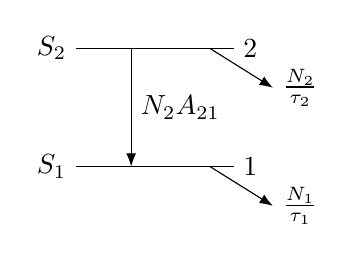
\begin{tikzpicture}
        \draw (0,0) node[anchor=east] {$S_1$} -- (2,0) node[anchor=west] {1};
        \draw (0,1.5) node[anchor=east] {$S_2$} -- (2,1.5) node[anchor=west] {2};
        \draw[-Latex] (0.7,1.5) -- (0.7,0) node[anchor=west,midway] {$N_2A_{21}$};
        \draw[-Latex] (1.7,1.5) -- (2.5,1) node[anchor=west] {$\frac{N_2}{\tau_2}$};
        \draw[-Latex] (1.7,0) -- (2.5,-0.5) node[anchor=west] {$\frac{N_1}{\tau_1}$};
    \end{tikzpicture}
\end{figure}
Develop rate equations for $N_1$ and $N_2$.
\begin{align}
    \frac{dN_2}{dt} &= S_2 - \frac{N_2}{\tau_2} \\
    \frac{dN_1}{dt} &= S_1 + N_2A_{21} - \frac{N_1}{\tau_1}
\end{align}
In the steady state, 
\begin{align}
    \frac{dN_2}{dt} &= \frac{dN_1}{dt} = 0 \\
    N_2 &= S_2\tau_2 \\
    N_1 &= S_1\tau_1 + A_{21}\tau_1N_2 \\
        &= S_1\tau_1 + A_{21}\tau_1S_2\tau_2
\end{align}
Population inversion density,
\begin{align}
    N_0^* &= N_2 - \frac{g_2}{g_1}N_1 \\
        &= S_2\tau_2\left(1-\frac{g_2}{g_1}A_{21}\tau_1\right) - \frac{g_2}{g_1}S_1\tau_1
\end{align}
'0' denotes small signal coefficient (in the absence of field).
\begin{multicols}{2}
\begin{figure}[H]
    \centering
    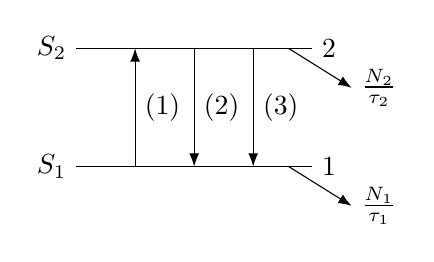
\begin{tikzpicture}
        \draw (0,0) node[anchor=east] {$S_1$} -- (3,0) node[anchor=west] {1};
        \draw (0,1.5) node[anchor=east] {$S_2$} -- (3,1.5) node[anchor=west] {2};
        \draw[-Latex] (0.75,0) -- (0.75,1.5) node[anchor=west,midway] {(1)};
        \draw[-Latex] (1.5,1.5) -- (1.5,0) node[anchor=west,midway] {(2)};
        \draw[-Latex] (2.25,1.5) -- (2.25,0) node[anchor=west,midway] {(3)};
        \draw[-Latex] (2.7,1.5) -- (3.5,1) node[anchor=west] {$\frac{N_2}{\tau_2}$};
        \draw[-Latex] (2.7,0) -- (3.5,-0.5) node[anchor=west] {$\frac{N_1}{\tau_1}$};
    \end{tikzpicture}
\end{figure}
\begin{align}
    (1)&~~ \frac{g_2}{g_1}N_1\sigma(\om)\frac{I}{\hbar\om}\\
    (2)&~~ N_2\sigma(\om)\frac{I}{\hbar\om} \\
    (3)&~~ N_2A_{21}
\end{align}
\end{multicols}
We have assumed $L(\om) < \Gamma_{21}$.
\begin{align}
    \frac{dN_2}{dt} &= S_2 - \frac{N_2}{\tau_2} - N^*\sigma(\om)\frac{I}{\hbar\om} \\
    \frac{dN_1}{dt} &= S_1 - \frac{N_1}{\tau_1} + N^*\sigma(\om)\frac{I}{\hbar\om} + A_{21}N_2 \\
    N_2 &= S_2\tau_2 - N^*\left(\frac{\sigma I}{\hbar\om}\right)\tau_2 \\
    N_1 &= S_1\tau_1 + N^*\left(\frac{\sigma I}{\hbar\om}\right)\tau_1 + A_{21}\tau_1N_2 \\
    N^* &= \frac{S_2\tau_2\left(1-\frac{g_2}{g_1}A_{21}\tau_1\right) - \frac{g_2}{g_1}S_1\tau_1}{1+\left(\frac{\sigma I}{\hbar\om}\right)\left[\tau_2+\frac{g_2}{g_1}\left(1-A_{21}\tau_2\right)\tau_1\right]}
\end{align}
Numerator is $N_0^*$:
\begin{align}
    N^* &= \frac{N_0^*}{1 + \frac{I}{I_s}}
\end{align}
We can now define Saturation Intensity:
\begin{align}
    I_s(\om) &= \frac{\hbar\om}{\sigma(\om)}\frac{1}{\tau_2+\frac{g_2}{g_1}\tau_1(1-A_{21}\tau_2)}
\end{align}
Gain is saturated too, since
\begin{align}
    g(\om) &= \sigma(\om)N^* = \frac{g_0(\om)}{1 + \frac{I}{I_s(\om)}}
\end{align}
\textbf{Comments:}
\begin{itemize}
    \item At $I = I_s(\om) \to g(\om) = \frac{g_0(\om)}{2}$.
    \item $I_s(\om)$ is frequency dependent through $\sigma(\om)$, so will happen quicker at line centre.
    \item For an efficient laser, expect large population inversion $\implies \tau_2 \gg \tau_1$.
    \item All decays from state 2 into state 1 $\implies A_{21} \approx \frac{1}{\tau_2}$.
\end{itemize}
\begin{align}
    I_s(\om) &= \frac{\hbar\om}{\sigma(\om)\tau_2}
\end{align}
This is usually an excellent approximation.
\begin{example}[Linear Amplifier]
    \begin{figure}[H]
        \centering
        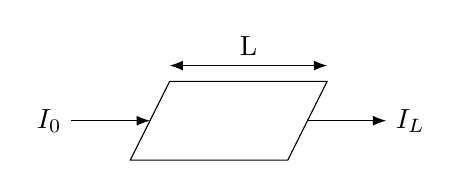
\begin{tikzpicture}
            \draw[-Latex] (0,1) node[anchor=east] {$I_0$} -- (1,1);
            \draw (0.75,0.5) -- (1.25,1.5) -- (3.25,1.5) -- (2.75,0.5) -- cycle;
            \draw[Latex-Latex] (1.25,1.7) -- (3.25,1.7) node[anchor=south,midway] {L};
            \draw[-Latex] (3,1) -- (4,1) node[anchor=west] {$I_L$};
        \end{tikzpicture}\vspace{-25pt}
    \end{figure}
    \begin{align}
        \frac{dI}{dz} &= g(\om)I = \frac{g_0(\om)I}{1 + \frac{I}{I_s(\om)}}
    \end{align}
    We just integrate this, after length L:
    \begin{align}
        \int_{I(0)}^{I(L)} \frac{1+\frac{I}{I_s(\om)}}{I}\,dI &= \int_0^L g_0(\om)\,dz \\
        \ln\left(\frac{I_L}{I_0}\right) + \frac{I_L-I_0}{I_s(\om)} &= g_0(\om)L
    \end{align}
    \textbf{Two limiting cases:}
    \begin{enumerate}
        \item $I/I_s(\om) \ll 1 \implies$ exponential growth,
            \begin{align}
                I_L &= I_0e^{g_0(\om)L}
            \end{align}
        \item $I/I_s(\om) \gg 1 \implies$ linear growth,
            \begin{align}
                I_L &= I_0  + g_0(\om)I_s(\om)L
            \end{align}
    \end{enumerate}
    \begin{figure}[H]
        \centering
        \begin{tikzpicture}
            \draw[->] (0,0) -- (0,2.5) node[anchor=east] {$I(z)$};
            \draw[->] (0,0) -- (4,0) node[anchor=north] {$z$};
            \draw (0,0.3) node[anchor=east] {$I_0$} parabola (2,1.2) -- (3.2,2.2);
            \draw[dashed] (2,1.2) -- (0.56,0);
            \draw[dashed] (0,0.3) -- (2,0.3);
        \end{tikzpicture}
    \end{figure}
\end{example}

\chapter{Multimode lasing and output power}
Last time:
\begin{align}
    \frac{dN_2}{dt} &= S_2 - \frac{N_2}{\tau_2} - \frac{N^*\sigma(\om)I}{\hbar\om} \\
    \frac{dN_1}{dt} &= S_1 - \frac{N_1}{\tau_1} + \frac{N^*\sigma(\om)I}{\hbar\om} + N_2A_{21} 
\end{align}
We need a third equation to describe the system.
Develop equation governing the the intensity build up. 
Consider photon density, $n_\phi$.
\begin{align}
    \frac{dn_\phi}{dt} &= \left(N^*\sigma(\om)\frac{I}{\hbar\om}\right)\left(\frac{L_m}{L_c}\right) - \frac{n_\phi}{\tau_c}
\end{align}
Intensity of beam, 
\begin{align}
    I &= \text{energy density}\times\text{velocity} \\
      &= n_\phi\hbar\om\times c \\
    n_\phi &= \frac{I}{\hbar\om c} \\
    dn_\phi &= \frac{I}{\hbar\om c}dI \\
    \frac{dI}{dt} &= N^*\sigma(\om)cI\left(\frac{L_m}{L_c}\right)-\frac{I}{\tau_c}
\end{align}
We know that
\begin{align}
    \tau_c &= \frac{2L_c}{c\delta_c} & g_{th} &= \frac{\delta_c}{2L_m}.
\end{align}
We then find the following useful for the final substitution:
\begin{align}
    \frac{1}{\tau_c} &= \frac{c\delta_c}{2L_c} = c\left(\frac{L_m}{L_c}\right)g_{th} \\
    g(\om) &= N^*\sigma(\om) \\
    \frac{dI}{dt} &= c\left(\frac{L_m}{L_c}\right)\left[g(\om) - g_{th}\right]I(t)
\end{align}
In the steady state, this should be zero which is found either if $I(t)$ is zero which is meaningless solution, or if $g_{ss}(\om) = g_{th}$.
This highlights the principle of gain saturation.
We can take the expression found for gain last time and apply the above relation.
\begin{multicols}{2}
\begin{figure}[H]
    \centering
    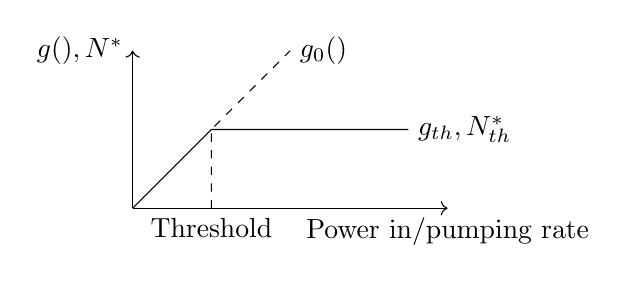
\begin{tikzpicture}
        \draw[->] (0,0) -- (0,2) node[anchor=east] {$g(\om),N^*$};
        \draw[->] (0,0) -- (4,0) node[anchor=north] {Power in/pumping  rate};
        \draw (0,0) -- (1,1) -- (3.5,1) node[anchor=west] {$g_{th},N_{th}^*$};
        \draw[dashed] (1,0) node[anchor=north] {Threshold} -- (1,1) -- (2,2) node[anchor=west] {$g_0(\om)$};
    \end{tikzpicture}
\end{figure}
\begin{align}
    g_{ss}(\om) &= \sigma(\om)N^* = \frac{g_0(\om)}{1+I_{ss}/I_s(\om)} = g_{th} \\
    I_{ss} &= I_s(\om)\left[\frac{g_0(\om)}{g_{th}}-1\right]
\end{align}
\end{multicols}
Consider simple cavity, 
\begin{figure}[H]
    \centering
    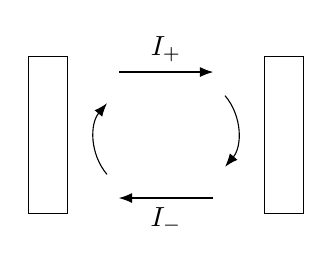
\begin{tikzpicture}
        \draw (0,0) rectangle (0.5,2);
        \draw (3,0) rectangle (3.5,2);
        \draw[-Latex] (1.15,1.8) -- (2.35,1.8) node[anchor=south,midway] {$I_+$};
        \draw[-Latex] (2.35,0.2) -- (1.15,0.2) node[anchor=north,midway] {$I_-$};
        \draw[-Latex] (1,0.5) arc (220:140:20pt);
        \draw[-Latex] (2.5,1.5) arc (40:-40:20pt);
    \end{tikzpicture}
\end{figure}
Mirror transmission, $T=(I-R),~ I_{out} = T\times I_+$.
Assume low output coupling-uniform field approximation, i.e. $I_+ \approx I_-$.
\begin{multicols}{2}
\begin{figure}[H]
    \centering
    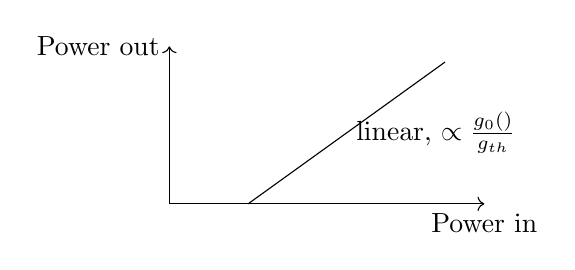
\begin{tikzpicture}
        \draw[->] (0,0) -- (0,2) node[anchor=east] {Power out};
        \draw[->] (0,0) -- (4,0) node[anchor=north] {Power in};
        \draw (1,0) -- (3.5,1.8) node[anchor=west,midway] {linear, $\propto \frac{g_0(\om)}{g_{th}}$};
    \end{tikzpicture}
\end{figure}
\begin{align}
    I_{ss} &= I_+ + I_- \approx 2I_+ \\
    I_{out} &= T\times \frac{I_{ss}}{2} = T\frac{I_s(\om)}{2}\left[\frac{g_0(\om)}{g_{th}}-1\right]
\end{align}
\end{multicols}
To get output power, we need to know mode area, $A_{mode}$.
\begin{align}
    P_{out} &= A_{mode}I_{out} = \frac12I_s(\om)A_{mode}T\left[\frac{g_0(\om)}{g_{th}}-1\right]
\end{align}

\section{Optimum Output Coupling}
\begin{multicols}{2}
\begin{figure}[H]
    \centering
    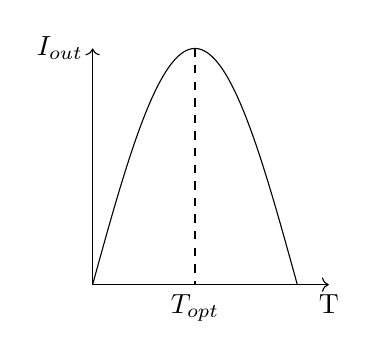
\begin{tikzpicture}
        \draw[->] (0,0) -- (0,3) node[anchor=east] {$I_{out}$};
        \draw[->] (0,0) -- (3,0) node[anchor=north] {T};
        \draw (0,0) sin (1.3,3) cos (2.6,0);
        \draw[dashed] (1.3,3) -- (1.3,0) node[anchor=north] {$T_{opt}$};
    \end{tikzpicture}
\end{figure}
\begin{align}
    I_{out} &= T\frac{I_s(\om)}{2}\left[\frac{g_0(\om)}{g_{th}}-1\right] \\
    g_{th} &= \frac{\delta_c}{2L_m},~ \delta_c = T+\delta_{loss} \\
    I_{out} &= T\frac{I_s(\om)}{2}\left[\frac{2g_0(\om)}{T+\delta_{loss}}-1\right]
\end{align}
\end{multicols}
Differentiate expression for $I_{out}$ with respect to T and set to zero:
\begin{align}
    \frac{dI_{out}}{dT} &= \frac{I_s(\om)}{2}\left[\frac{2g_0(\om)}{T+\delta_{loss}}-1\right] - \frac{TI_s(\om)}{2}\frac{2g_0(\om)L}{(T+\delta_{loss})^2} \\
    2g_0(\om)L(T+\delta_{loss}) &- (T+\delta_{loss})^2 = 2g_0(\om)LT \\
    (T+\delta_{loss})^2 &= 2g_0(\om)L\delta_{loss} \\
    T_{opt} &= \sqrt{2g_0(\om)L\delta_{loss}} - \delta_{loss} \\
    I_{opt} &= \left[1-\left(\frac{\delta_{loss}}{2g_0(\om)L}\right)^{1/2}\right]^2 g_0(\om)LI_s(\om) \\
    I_{max} &= g_0(\om)LI_s(\om)
\end{align}

\chapter{Requirements for Population Inversion}
\section{Condition for Steady State Population Inversion}
\begin{figure}[H]
    \centering
    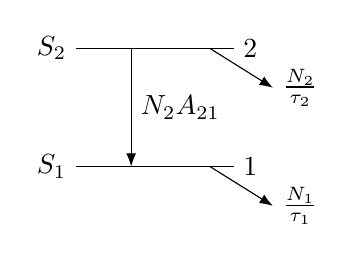
\begin{tikzpicture}
        \draw (0,0) node[anchor=east] {$S_1$} -- (2,0) node[anchor=west] {1};
        \draw (0,1.5) node[anchor=east] {$S_2$} -- (2,1.5) node[anchor=west] {2};
        \draw[-Latex] (0.7,1.5) -- (0.7,0) node[anchor=west,midway] {$N_2A_{21}$};
        \draw[-Latex] (1.7,1.5) -- (2.5,1) node[anchor=west] {$\frac{N_2}{\tau_2}$};
        \draw[-Latex] (1.7,0) -- (2.5,-0.5) node[anchor=west] {$\frac{N_1}{\tau_1}$};
    \end{tikzpicture}\vspace{-25pt}
\end{figure}
Develop rate equations for $N_1$ and $N_2$.
\begin{align}
    \frac{dN_2}{dt} &= S_2 - \frac{N_2}{\tau_2} \\
    \frac{dN_1}{dt} &= S_1 + N_2A_{21} - \frac{N_1}{\tau_1} 
\end{align}
In steady state, 
\begin{align}
    N_2 &= \tau_2S_2 \\
    N_1 &= \tau_1S_1 + \tau_2S_2A_{21}\tau_1
\end{align}
For population inversion, $N^* > 0$, or $\frac{N_2}{g_2} > \frac{N_1}{g_1}$.
\begin{align}
    \frac{\tau_2S_2}{g_2} &> \frac{\tau_1S_1}{g_1} + \frac{\tau_2S_2A_{21}\tau_1}{g_1} \\
    1 &< \frac{g_1}{g_2}\frac{S_2\tau_2}{S_1\tau_1}\left[1-\frac{g_2}{g_1}A_{21}\tau_1\right]
\end{align}
We want:
\begin{itemize}
    \item $S_2 > S_1$ - selective pumping
    \item $\tau_2 > \tau_1$ - favourable lifetime ratio
    \item $g_1 > g_2$ - favourable degeneracy ratio
    \item The term in the square brackets only depends on the atomic properties, and we require
        \begin{align}
            A_{21} < \frac{g_1}{g_2}\frac{1}{\tau_1}
        \end{align}
        to be able to get laser oscillation.
        This is the \textbf{minimum} requirement for steady state inversion - alone, it may not be a sufficient condition, but it is necessary.
        The lower laser level must decay faster than it is being filled by spontaneous emission.
\end{itemize}

\section{Three and Four Level Lasers}
\subsection{Traditional Solid State Three-level Laser}
\begin{figure}[H]
    \centering
    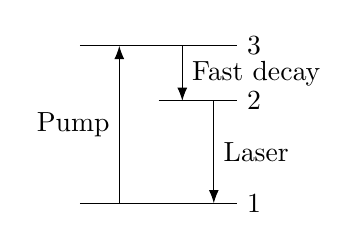
\begin{tikzpicture}
        \draw (0,0) -- (2,0) node[anchor=west] {1};
        \draw (1,1.3) -- (2,1.3) node[anchor=west] {2};
        \draw (0,2) -- (2,2) node[anchor=west] {3};
        \draw[-Latex] (0.5,0) -- (0.5,2) node[anchor=east,midway] {Pump};
        \draw[-Latex] (1.3,2) -- (1.3,1.3) node[anchor=west,midway] {Fast decay}; 
        \draw[-Latex] (1.7,1.3) -- (1.7,0) node[anchor=west,midway] {Laser};
    \end{tikzpicture}
\end{figure}
This is known as the traditional solid state three-level laser, e.g. Ruby. 

\subsection{Gas lasers}
\begin{figure}[H]
    \centering
    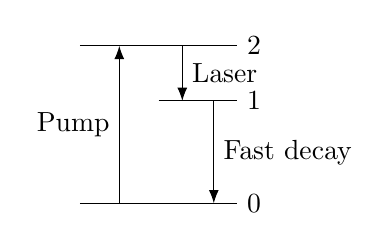
\begin{tikzpicture}
        \draw (0,0) -- (2,0) node[anchor=west] {0};
        \draw (1,1.3) -- (2,1.3) node[anchor=west] {1};
        \draw (0,2) -- (2,2) node[anchor=west] {2};
        \draw[-Latex] (0.5,0) -- (0.5,2) node[anchor=east,midway] {Pump};
        \draw[-Latex] (1.3,2) -- (1.3,1.3) node[anchor=west,midway] {Laser};
        \draw[-Latex] (1.7,1.3) -- (1.7,0) node[anchor=west,midway] {Fast decay};
    \end{tikzpicture}
\end{figure}
This is common for gas lasers, e.g. Ar+.

\subsection{Solid state and dye lasers}
\begin{figure}[H]
    \centering
    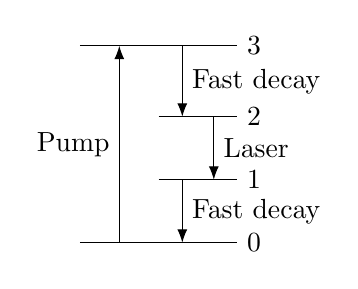
\begin{tikzpicture}
        \draw (0,0) -- (2,0) node[anchor=west] {0};
        \draw (1,0.8) -- (2,0.8) node[anchor=west] {1};
        \draw (1,1.6) -- (2,1.6) node[anchor=west] {2};
        \draw (0,2.5) -- (2,2.5) node[anchor=west] {3};
        \draw[-Latex] (0.5,0) -- (0.5,2.5) node[anchor=east,midway] {Pump};
        \draw[-Latex] (1.3,2.5) -- (1.3,1.6) node[anchor=west,midway] {Fast decay};
        \draw[-Latex] (1.7,1.6) -- (1.7,0.8) node[anchor=west,midway] {Laser};
        \draw[-Latex] (1.3,0.8) -- (1.3,0) node[anchor=west,midway] {Fast decay};
    \end{tikzpicture}
\end{figure}
This is most solid state lasers and dye lasers, e.g. Nd:YAG.

\subsection{General comments}
\begin{itemize}
    \item We only show three/four levels here but each one of these levels may be a tight collection of thousands of levels which may be close enough to be treated as a single big level.
    \item For three-level schemes, one transition must be non-radiative to conserve parity.
        \begin{itemize}
            \item For three-level solid state lasers, there is fast phonon decay from 3 to 2.
            \item For gas lasers, both downward transitions are radiative but pumping is achieved by collisions.
        \end{itemize}
    \item Traditional sold state laser will have a high pumping threshold because we need to transfer $\frac{N}{2}$ out of state 1 to get inversion, so these are not very efficient.
    \item Gas lasers have a low \emph{quantum efficiency}.
        \begin{equation}
            Q.E. = \frac{E_2-E_1}{E_2-E_0} = \frac{\text{laser photon energy}}{\text{pump 'photon' energy}} = \frac{\hbar\om_{12}}{\hbar\om_{20}}
        \end{equation}
        because spontaneous emission rate $A_{21}\propto\om_{12}^3$, hence to achieve $\tau_2>\tau_1$ requires $\om_{10}>\om_{12}$.
    \item Four-level lasers are best, \emph{cause bigger is better, baybeeeee.}
\end{itemize}
\begin{align}
    \text{Gain} &= e^{g(\om)L} = e^{\sigma(\om)N^*L_m}
\end{align}
$\sigma(\om)$ and $L_m$ are fixed (or practically so), so for us to maximise our gain, we have to maximise $N^*$ through pumping. 

\section{Three-Level Traditional Solid State Lasers}
\begin{figure}[H]
    \centering
    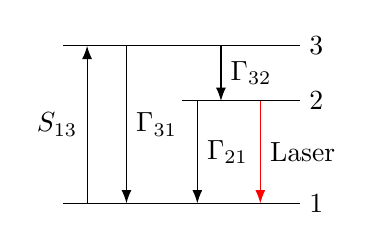
\begin{tikzpicture}
        \draw (0,0) -- (3,0) node[anchor=west] {1};
        \draw (1.5,1.3) -- (3,1.3) node[anchor=west] {2};
        \draw (0,2) -- (3,2) node[anchor=west] {3};
        \draw[-Latex] (0.3,0) -- (0.3,2) node[anchor=east,midway] {$S_{13}$};
        \draw[-Latex] (2,2) -- (2,1.3) node[anchor=west,midway] {$\Gamma_{32}$};
        \draw[-Latex,red] (2.5,1.3) -- (2.5,0) node[anchor=west,midway,black] {Laser};
        \draw[-Latex] (0.8,2) -- (0.8,0) node[anchor=west,midway] {$\Gamma_{31}$};
        \draw[-Latex] (1.7,1.3) -- (1.7,0) node[anchor=west,midway] {$\Gamma_{21}$};
    \end{tikzpicture}
\end{figure}
To study the steady state small signal population inversion, we ignore the effects of the laser field on the populations. 
The rate equations are:
\begin{align}
    \frac{dN_3}{dt} &= S_{13}N_1 - (\Gamma_{31}+\Gamma_{32})N_3 \\
    \frac{dN_2}{dt} &= \Gamma_{32}N_3 - \Gamma_{21}N_2 \\
    \frac{dN_1}{dt} &= -S_{13}N_1 + \Gamma_{31}N_1 + \Gamma_{21}N_2
\end{align}

\chapter{Population Inversion in Four-level lasers}
\begin{figure}[H]
    \centering
    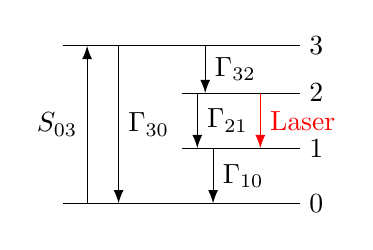
\begin{tikzpicture}
        \draw (0,0) -- (3,0) node[anchor=west] {0};
        \draw (1.5,0.7) -- (3,0.7) node[anchor=west] {1};
        \draw (1.5,1.4) -- (3,1.4) node[anchor=west] {2};
        \draw (0,2) -- (3,2) node[anchor=west] {3};
        \draw[-Latex] (0.3,0) -- (0.3,2) node[anchor=east,midway] {$S_{03}$};
        \draw[-Latex] (0.7,2) -- (0.7,0) node[anchor=west,midway] {$\Gamma_{30}$};
        \draw[-Latex] (1.8,2) -- (1.8,1.4) node[anchor=west,midway] {$\Gamma_{32}$};
        \draw[-Latex,red] (2.5,1.4) -- (2.5,0.7) node[anchor=west,midway] {Laser};
        \draw[-Latex] (1.7,1.4) -- (1.7,0.7) node[anchor=west,midway] {$\Gamma_{21}$};
        \draw[-Latex] (1.9,0.7) -- (1.9,0) node[anchor=west,midway] {$\Gamma_{10}$};
    \end{tikzpicture}
\end{figure}
$\Gamma_{32}$ is a fast, non-radiative decay; $\Gamma_{10}$ likewise.
\begin{align}
    \frac{dN_3}{dt} &= N_0S_{03} - \left(\Gamma_{30}+\Gamma_{32}\right)N_3 \\
    \frac{dN_2}{dt} &= N_3\Gamma_{32} - N_2\Gamma_{21} \\
    \frac{dN_1}{dt} &= N_2\Gamma_{21} - N_1\Gamma_{10} \\
    \frac{dN_0}{dt} &= -N_0S_{03} + N_3\Gamma_{30} + N_1\Gamma_{10}
\end{align}
In the ideal case, $\Gamma_{32}\gg\Gamma_{30}$, and $N_3\approx0$, i.e. decay is faster than pumping.

\section{Idealised Four-level laser}
\begin{figure}[H]
    \centering
    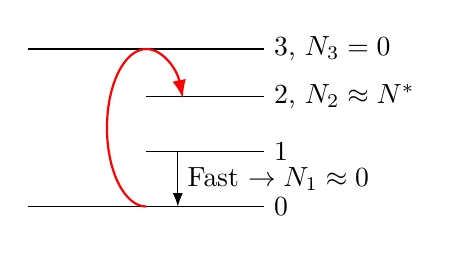
\begin{tikzpicture}
        \draw (0,0) -- (3,0) node[anchor=west] {0};
        \draw (1.5,0.7) -- (3,0.7) node[anchor=west] {1};
        \draw (1.5,1.4) -- (3,1.4) node[anchor=west] {2, $N_2\approx N^*$};
        \draw (0,2) -- (3,2) node[anchor=west] {3, $N_3=0$};
        \draw[-Latex] (1.9,0.7) -- (1.9,0) node[anchor=west,midway] {Fast $\to N_1\approx0$};
        \draw[thick,red,-Latex] (1.5,1) [partial ellipse=270:22:0.5cm and 1cm];
    \end{tikzpicture}
\end{figure}
The idealised four-level laser equations:
\begin{align}
    N_0 &\approx N & N_2 &\approx \frac{S_{03}}{\Gamma_{21}}N & N_1 & N_3 = 0
\end{align}

\section{Comparison of three- and four-level laser schemes}
\begin{multicols}{2}
For a three-level scheme, we found that,
\begin{align}
    S_{12}^{th} &= \frac{N+N_{th}^*}{N-N_{th}^*}\Gamma_{21} \approx \Gamma_{21}.
\end{align}
For four-level schemes, we found that
\begin{align}
    S_{03}^{th} &= \frac{N_{th}^*}{N-N_{th}}\Gamma_{21} \approx \frac{N_{th}^*}{N}\Gamma_{21}
\end{align}
\end{multicols}
If we assume equal $\Gamma_{21}$s,
\begin{align}
    \frac{\text{four-level}}{\text{three-level}} &= \frac{S_{03}^{th}}{S_{13}^{th}} = \frac{N_{th}^*}{N+N_{th}^*} \approx \frac{N_{th}^*}{N} \ll 1
\end{align}
This reiterates that four-level lasers are much more efficient than three-level ones.
Comparing power per unit volume absorbed at threshold:
\begin{align}
    \left(\frac{P}{V}\right)_{th,3} &= \hbar\om_{13}\Gamma_{21}\frac{N}{2} & \left(\frac{P}{V}\right)_{th,4} &= \hbar\om_{30}N^*\Gamma_{21}
\end{align}

\begin{example}[Ruby vs Nd:YAG]
    Ruby doped at 1\% by weight.
    \begin{align}
        N_0 &= 3.3\times10^{26}\,m^{-3} & \Gamma_{21} &= 3.3\times10^2\,s^{-1}
    \end{align}
    Assume pumping at $\lambda=505\,nm$.
    Laser rod, diameter $6\,mm$, length $10\,cm$.
    \begin{align}
        P_{th} &= \left(\frac{hc}{\lambda}\right)\frac{N_0}{2}\Gamma_{21}\times V \approx 5.4\,kW
    \end{align}
    Now for the ND:YAG,
    \begin{align}
        \Gamma_{21} &= 1.8\times10^3\,s^{-1} & \sigma &= 9\times10^{-19}\,cm^2 
    \end{align}
    Assume cavity loss of $\delta_c = 0.05$, with diameter $4\,mm$, and length $5\,cm$.
    Pumped at $808\,nm$.
    \begin{align}
        N_{th}^* &= \frac{\delta_c}{2\sigma L_m} = 5.6\times10^{21}\,m^{-3} \\
        P_{th} &= \hbar\om_{30}N_{th}^*\Gamma_{21}V \approx 1.66\,W
    \end{align}
    So Ruby has a massive energy cost compared to Nd:YAG, Nd:YAG much preferable.
\end{example}

\chapter{Population Inversion in Three-level Gas Lasers}
\begin{figure}[H]
    \centering
    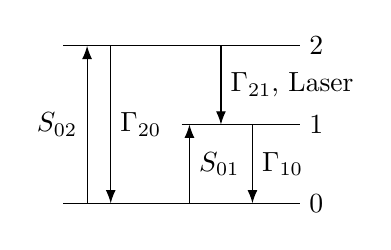
\begin{tikzpicture}
        \draw (0,0) -- (3,0) node[anchor=west] {0};
        \draw (1.5,1) -- (3,1) node[anchor=west] {1};
        \draw (0,2) -- (3,2) node[anchor=west] {2};
        \draw[-Latex] (0.3,0) -- (0.3,2) node[anchor=east,midway] {$S_{02}$};
        \draw[-Latex] (0.6,2) -- (0.6,0) node[anchor=west,midway] {$\Gamma_{20}$};
        \draw[-Latex] (2,2) -- (2,1) node[anchor=west,midway] {$\Gamma_{21}$, Laser};
        \draw[-Latex] (1.6,0) -- (1.6,1) node[anchor=west,midway] {$S_{01}$};
        \draw[-Latex] (2.4,1) -- (2.4,0) node[anchor=west,midway] {$\Gamma_{10}$};
    \end{tikzpicture}
\end{figure}
Develop rate equations in absence of field:
\begin{align}
    \frac{dN_2}{dt} &= S_{02}N_0 - (\Gamma_{20}+\Gamma_{21})N_2 \\
    \frac{dN_1}{dt} &= S_{01}N_0 + \Gamma_{21}N_2 - \Gamma_{10}N_1 \\
    \frac{dN_0}{dt} &= -(S_{02}+S_{01})N_0 + \Gamma_{20}N_2 + \Gamma_{10}N_1
\end{align}
Using the steady state definition, $\frac{dN_i}{dt}=0$:
\begin{align}
    N_2 &= \frac{S_{02}}{\Gamma_{20}+\Gamma_{21}}N_0 \\
    S_{01}N_0 &+ \Gamma_{21}\left[\frac{S_{02}}{\Gamma_{20}+\Gamma_{21}}N_0\right] - \Gamma_{10}N_1 = 0 \\
    N_1 &= \frac{S_{01}(\Gamma_{20}+\Gamma_{21})+\Gamma_{21}S_{02}}{\Gamma_{10}(\Gamma_{20}+\Gamma_{21})}N_0
\end{align}
For population inversion, we need
\begin{align}
    \frac{N_2}{N_1} &> \frac{g_2}{g_1} \\
    N^* &= N_2 - \frac{g_2}{g_1}N_1 > 0 \\
    \frac{N_2}{N_1} &= \frac{S_{02}\Gamma_{10}}{S_{01}(\Gamma_{20}+\Gamma_{21})+\Gamma_{21}S_{02}} > \frac{g_2}{g_1}
\end{align}
We have to find another pumping technique as we cannot use light. 
Both down transitions are optical (radiative), so $S_{02}$ cannot be optical due to parity conservation, and $\Gamma_{20}$ is negligible.
\begin{align}
    \frac{N_2}{N_1} &= \frac{S_{02}\Gamma_{10}}{(S_{01}+S_{02})\Gamma_{21}} > \frac{g_2}{g_1} \\
    \frac{S_{02}}{S_{01}} &> \left(\frac{g_1\Gamma_{10}}{g_2\Gamma_{21}}-1\right)^{-1}
\end{align}

\begin{example}[Argon ion laser]
    \begin{wrapfigure}{l}{0.25\textwidth}
        \centering
        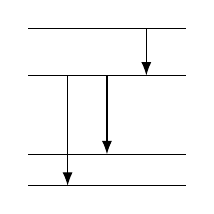
\begin{tikzpicture}
            \draw (0,0) -- (2,0);
            \draw (0,0.4) -- (2,0.4);
            \draw (0,1.4) -- (2,1.4);
            \draw (0,2) -- (2,2);
            \draw[-Latex] (1,1.4) -- (1,0.4);
            \draw[-Latex] (0.5,1.4) -- (0.5,0);
            \draw[-Latex] (1.5,2) -- (1.5,1.4);
        \end{tikzpicture}
    \end{wrapfigure}
    \textit{doodle the diagram, (laser) 488.0 nm with A = 7.8x10to7 s-1, (decays) 73.1nm A = 4.5x10to8 s-1, 72.3nm A = 23x10to8 s-1}
    We have a degeneracy of $g = 2J+1$, so $g_1 = 4, g_2 = 6$.
    $\Gamma_{21} = 7.8\times10^7\,s^{-1}$, $\Gamma_{10}=27.5\times10^8\,s^{-1}$.\\
    From this, we get a ratio of $0.044$.
    For this particular system, we can pump into the lower level 22.5 times as quickly as into the upper one and still maintain population inversion due to fast natural decay rates.
    \textbf{Striking result!}\\
    This can happen because $A \propto \om^3$ so massively different for the higher frequencies of the lower level decay.
    The downside is low quantum efficiency.
\end{example}
Gas lasers cannot be optically pumped, so they use collisions, or \textbf{particle pumping.}

\chapter{The Fabry-Perot Etalon and Laser Cavity Modes}
\textit{write initial bit up from slides}

\section{The Fabry-Perot Elaton}
\begin{align}
    \frac{I_T}{I_0} &= \frac{T^2}{(1-R)^2}\frac{1}{1+\frac{4F^2}{\pi^2}\sin^2\frac{\delta}{2}}
\end{align}
\textit{doodle Airy pattern in slides}\\
Points to note:
\begin{itemize}
    \item For mirrors, $T+R+A = 1$, absorption $A\approx0$, so $T=1-R$.
        \begin{align}
            \frac{I_T}{I_0}\bigg|_{max} &= 1
        \end{align}
        So all light trnasmitted at cavity resonance.
    \item Phase difference:
        \begin{align}
            \delta &= \frac{4\pi d}{\lambda}\cos\theta
        \end{align}
        Dependent on angle, separation, and wavelength. 
    \item For bright fringes, $\sin\frac{\delta}{2}=0$ so $\delta=2n\pi$, or $2d\cos\theta = n\lambda$.
    \item Free spectral range, $\Delta\nu_{fsr}$. At maxima, 
        \begin{align}
            \lambda &= \frac{2d\cos\theta}{n} \implies \nu = \frac{c}{\lambda} = \frac{nc}{\cos\theta} \\
            \Delta\nu_{fsr} &= \nu_{n+1}-\nu_n = \frac{c}{2d\cos\theta}
        \end{align}
        Then, at normal incidence, 
        \begin{align}
            \Delta\nu_{fsr} &= \frac{c}{2d}
        \end{align}
    \item Fringe width. What is the full width at half maximum (FWHM) of fringes? Assume $\frac{I_T}{I_0}=\frac12$ when $\delta=2\pi n\pm\delta_{1/2}$.
        \begin{align}
            \frac12 &= \frac{1}{1+\frac{4F^2}{\pi^2}\sin^2(\frac{\delta_{1/2}}{2})} \\
            \sin^2\left(\frac{\delta_{1/2}}{2}\right) &= \frac{\pi^2}{4F^2} \\
            \delta_{1/2} &= 2\sin^{-1}\left(\frac{\pi}{2F}\right) \\
            \delta_{1/2} &\approx \frac{\pi}{F},\; F >> 1 \\
            \text{FWHM} &= 2\delta_{1/2} = \frac{2\pi}{F}
        \end{align}
        Separation of adjacent peaks (in radians) $=2\pi$.
        Hence, finesse, 
        \begin{align}
            F &= \frac{\Delta\nu_{fsr}}{\Delta\nu_{FWHM}}
        \end{align}
        \textit{doodle it}\\
        So high finesse $\to$ sharp fringes, and vice versa.
        Before, 
        \begin{align}
            F &= \frac{\pi\sqrt{R}}{1-R} \implies \Delta\nu_{FWHM} = \frac{c}{2d}\left(\frac{1-R}{\pi\sqrt{R}}\right)
        \end{align}
\end{itemize}

\begin{example}
    30cm long etalon with mirrors, $R=0.99$.
    \begin{align}
        \Delta\nu_{fsr} &= \frac{c}{2d} = 500\,MHz \\
        F &= \frac{\pi\sqrt{R}}{1-R} \approx 313 \\
        \Delta\nu_{FWHM} &= \frac{\Delta\nu_{fsr}}{F} = 1.6\,MHz
    \end{align}
    In visible range, say $\lambda=550\,nm,~ \nu =  545\,THz$.
    We can use this etalon to reolve to 1 part in $10^8$.
\end{example}

\section{Laser Cavities}
The Fabry-Perot etalon is not a good laser cavity.
We need to place a gain medium between mirrors. 
\textit{doodle}
This cavity however is difficult to align.
More fundamentally, diffraction will cause losses.
\textit{doodle}
Diffraction leads to large losses.
The solution is to use curved mirrors: \textit{doodle}
Each curved mirror acts as a lens, \textit{doodle}
\begin{align}
    f &= \frac{R}{2}
\end{align}
where here R is the radius of curvature.
Cavity acts as a sequence of lenses.
\textit{doodle}
Related by Fourier transform, so essentially we want a function that is its own Fourier transform - Gauss-Hermite. 




\end{document}















